\documentclass[10pt]{article}

% Pacotes extras necessários
\usepackage{amsmath}
\usepackage[lmargin=0.5in, rmargin=0.5in, tmargin=0.5in, bmargin=0.5in, includehead, includefoot]{geometry}
\usepackage{amsfonts}
\usepackage[utf8]{inputenc}
\usepackage[portuguese]{babel}
\usepackage{graphicx}
\usepackage{fancyhdr}
\usepackage{setspace}
\usepackage{listings}
\usepackage{url}
\usepackage{enumitem}
\usepackage{appendix}
\usepackage{subcaption}
\usepackage[dvipsnames]{xcolor}
\usepackage{tikz}
\usetikzlibrary{positioning}

% Define estilo para listagens de código
\lstdefinestyle{mystyle}{
    language=Matlab,
    inputencoding=latin1,
    extendedchars=true,
    backgroundcolor=\color{white},
    basicstyle=\ttfamily\footnotesize,
    numbers=left,
    numberstyle=\tiny\color{gray},
    numbersep=5pt,
    tabsize=2,
    breaklines=true,
    keywordstyle=\color{blue},
    commentstyle=\color{green!60!black},
    stringstyle=\color{orange},
    frame=single,
    keepspaces=true,
    showspaces=false,
    showstringspaces=false,
    showtabs=false,
}
\lstset{style=mystyle}

\graphicspath{{./images/}}

\setlength{\parindent}{0pt}
\setstretch{1.5}

\DeclareMathOperator{\sen}{sen}
\DeclareMathOperator{\sinc}{sinc}
\newcommand{\Lap}[1]{\mathcal{L}\left\{#1\right\}}
\newcommand{\bm}[1]{\boldsymbol{#1}}

% Cabeçalho e rodapé em todas as páginas
\pagestyle{fancy}
\fancyhf{}
\fancyhead[L]{Relatório das simulações}
\fancyfoot[C]{\thepage}

% Dados do Grupo
\title{
    Trabalho Nº1 - MRAC Direto \\
    \large COE603 - Controle Adaptativo
}
\author{
    Caio Cesar Leal Verissimo - 119046624 \\
    Leonardo Soares da Costa Tanaka - 121067652 \\
    Lincoln Rodrigues Proença - 121076407 \\
    Engenharia de Controle e Automação - UFRJ \\
    Rio de Janeiro, Rio de Janeiro, Brasil \\
    Maio de 2025
}
\date{}

\begin{document}

\maketitle

% Geração automática do sumário
\tableofcontents
\newpage

\section{Resumo das equações do sistema}

Neste experimento, simulamos o algoritmo \textbf{MRAC Direto} para o caso:
\begin{itemize}
    \item $n = 1$ \hfill (ordem da planta)
    \item $n^* = 1$ \hfill (grau relativo)
    \item $n_p = 2$ \hfill (número de parâmetros)
\end{itemize}

\subsection{Equações do Algoritmo MRAC Direto}

A Tabela \ref{tab:equacoes_mrac} resume as equações fundamentais do algoritmo MRAC (Model Reference Adaptive Control) na forma direta, considerando uma planta de primeira ordem ($n = 1$), grau relativo igual a 1 ($n^* = 1$) e número de parâmetros $n_p = 2$.

\begin{table}[h!]
\centering
\begin{tabular}{|l|l|c|}
\hline
\textbf{Descrição}      & \textbf{Equação}                                  & \textbf{Ordem} \\ \hline
Planta                  & $\dot{y} = a_p y + k_p u$                         & 1              \\ \hline
Modelo                  & $\dot{y}_m = -a_m y_m + k_m r$                    & 1              \\ \hline
Erro da saída           & $e_0 = y - y_m$                                   &                \\ \hline
Lei de controle         & $u = \theta^T \omega$                  &                \\ \hline
Regressor               & $\omega^T = \begin{bmatrix} y & r \end{bmatrix}$ &                \\ \hline
Lei de adaptação        & $\dot{\theta} = -\text{sign}(k_p)\Gamma \omega e_0$ & 2 \\ \hline
\end{tabular}
\caption{Resumo do Algoritmo MRAC Direto}
\label{tab:equacoes_mrac}
\end{table}

A Figura \ref{fig:bloco_verificacao} ilustra o diagrama de blocos do sistema em malha fechada, juntamente com a verificação da equivalência com o modelo de referência. Este diagrama mostra como a combinação dos ganhos adaptativos $\theta_1^*$ e $\theta_2^*$ pode transformar o comportamento da planta para que ela imite o modelo de referência.

\begin{figure}[h!]
    \centering
    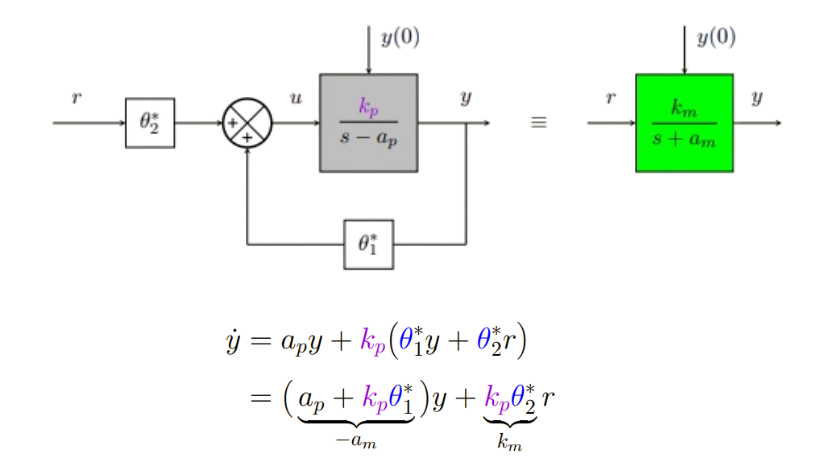
\includegraphics[width=0.6\textwidth]{img/diagrama.png}
    \caption{Diagrama de blocos e verificação da equivalência com o modelo de referência}
    \label{fig:bloco_verificacao}
\end{figure}

As expressões ideais para os parâmetros $\theta_1^*$ e $\theta_2^*$ que garantem essa equivalência são apresentadas a seguir. Esses parâmetros são obtidos por identificação direta, com base nas constantes do modelo e da planta.

\begin{center}
\begin{minipage}{0.45\textwidth}
\begin{center}
\fbox{
    $\theta_1^* = -\dfrac{a_p + a_m}{k_p}$
}
\end{center}
\end{minipage}
\begin{minipage}{0.45\textwidth}
\begin{center}
\fbox{
    $\theta_2^* = \dfrac{k_m}{k_p}$
}
\end{center}
\end{minipage}
\end{center}

Essas equações representam os valores ideais dos parâmetros adaptativos para que a planta controlada siga o comportamento especificado pelo modelo de referência. Na prática, o algoritmo de adaptação busca aproximar esses valores ao longo do tempo.

\subsection{Estabilidade do Algoritmo MRAC Direto}

\paragraph{1. Forma vetorial e definições}
Escrevendo em forma vetorial:
\begin{equation}
  \bm{\theta}^* = 
  \begin{bmatrix}
    \theta_1^* \\ \theta_2^*
  \end{bmatrix},
  \quad
  \bm{\omega} = 
  \begin{bmatrix}
    y \\ r
  \end{bmatrix}
  \quad\Longrightarrow\quad
  u^* = \bm{\theta}^{*T}\,\bm{\omega}.
\end{equation}
Analogamente, a lei de controle é
\begin{equation}
  \bm{\theta} = 
  \begin{bmatrix}
    \theta_1 \\ \theta_2
  \end{bmatrix}
  \quad\Longrightarrow\quad
  u = \bm{\theta}^T\,\bm{\omega}.
\end{equation}

\paragraph{2. Dinâmica do erro}
Definimos o erro de saída:
\begin{equation}
  e = y - y_m.
\end{equation}
Subtraindo as dinâmicas da planta e do modelo:
\begin{equation}
  \begin{aligned}
  \dot e 
  &= \dot y - \dot y_m
   = (a_p y + k_p u) - (-a_m y_m + k_m r) \\
  &= -a_m (y - y_m) + (a_p + a_m) y + k_p u - k_m r
    + \underbrace{(a_m y) - (a_m y)}_{=0} \\
  &= -a_m e
    + k_p\Bigl[\tfrac{a_p + a_m}{k_p}\,y + u - \tfrac{k_m}{k_p}\,r\Bigr] \\
  &= -a_m e + k_p \bigl[u - \theta_1^* y - \theta_2^* r\bigr] \\
  &= -a_m e + k_p \bigl[u - u^*\bigr].
  \end{aligned}
\end{equation}

\paragraph{3. Erro paramétrico}
Definimos o vetor de erro de parâmetro:
\begin{equation}
  \tilde{\bm{\theta}}
  = \bm{\theta} - \bm{\theta}^*
  \quad\Longrightarrow\quad
  \dot e = -a_m e + k_p\,\tilde{\bm{\theta}}^T\,\bm{\omega}.
\end{equation}

\paragraph{4. Função de Lyapunov}
Escolhemos
\begin{equation}
  V(e,\tilde{\bm{\theta}})
  = \tfrac12 e^2 + \tfrac12\,|k_p|\,\tilde{\bm{\theta}}^T\,\Gamma^{-1}\,\tilde{\bm{\theta}}.
\end{equation}
Calculando sua derivada:
\begin{equation}
  \begin{aligned}
  \dot V
  &= e\,\dot e
   + |k_p|\,\tilde{\bm{\theta}}^T\,\Gamma^{-1}\,\dot{\tilde{\bm{\theta}}} \\
  &= -a_m e^2
     + k_p\,\tilde{\bm{\theta}}^T\,\bm{\omega}\,e
     + |k_p|\,\tilde{\bm{\theta}}^T\,\Gamma^{-1}\,\dot{\tilde{\bm{\theta}}}.
  \end{aligned}
\end{equation}
Para garantir $\dot V\le0$, adotamos a lei de adaptação
\begin{equation}
  \dot{\bm{\theta}}
  = -\Gamma\,\mathrm{sign}(k_p)\,\bm{\omega}\,e.
\end{equation}

\paragraph{5. Conclusões de estabilidade}
Com essa escolha,
\begin{equation}
  \dot V = -a_m e^2 \le 0,
  \quad\Longrightarrow\quad
  e(t),\;\tilde{\bm{\theta}}(t)\;\in\mathcal L_\infty.
\end{equation}
Como $r(t)\in\mathcal L_\infty\Rightarrow y_m(t)\in\mathcal L_\infty$ e
\begin{equation}
  \dot V \le0 \;\Longrightarrow\; V(t)\le V(0),
\end{equation}
segue que
\begin{equation}
  \int_0^t e^2(\tau)\,d\tau < \infty
  \quad\Longrightarrow\quad
  e \in \mathcal L_2.
\end{equation}
Finalmente, aplicando o lema de Barbalat,
\begin{equation}
  e\in\mathcal L_2,\quad \dot e\in\mathcal L_\infty
  \quad\Longrightarrow\quad
  \lim_{t\to\infty} e(t) = 0.
\end{equation}

\section{Diagramas de blocos}

Nesta seção, apresentamos os principais diagramas de blocos que descrevem o funcionamento do controle adaptativo modelo-referência (MRAC) na sua forma direta. Cada figura ilustra uma parte fundamental do sistema, desde a estrutura geral até os componentes individuais como a planta, o modelo de referência e a malha de adaptação.

\begin{figure}[h!]
  \centering
  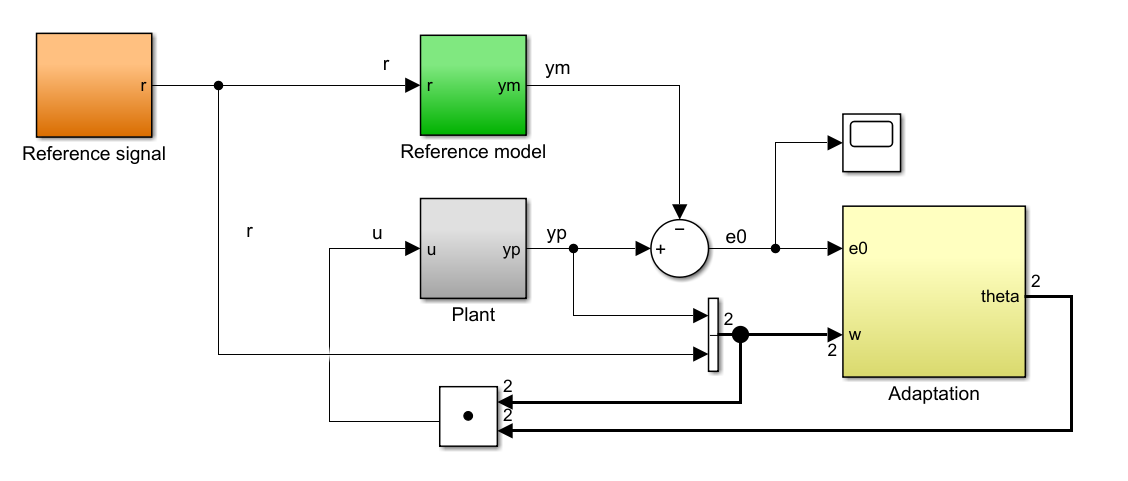
\includegraphics[width=0.8\textwidth]{img/diagrama_mrac_direto.png}
  \caption{Diagrama de blocos geral do controle MRAC direto.}
  \label{fig:mrac_direto}
\end{figure}

A Figura~\ref{fig:mrac_direto} mostra a arquitetura geral do controlador MRAC direto. O objetivo do sistema é ajustar os parâmetros do controlador de modo que a saída da planta acompanhe a saída do modelo de referência para qualquer entrada $r(t)$. O sinal de erro $e = y - y_m$ é utilizado para atualizar os parâmetros adaptativos.

\begin{figure}[h!]
  \centering
  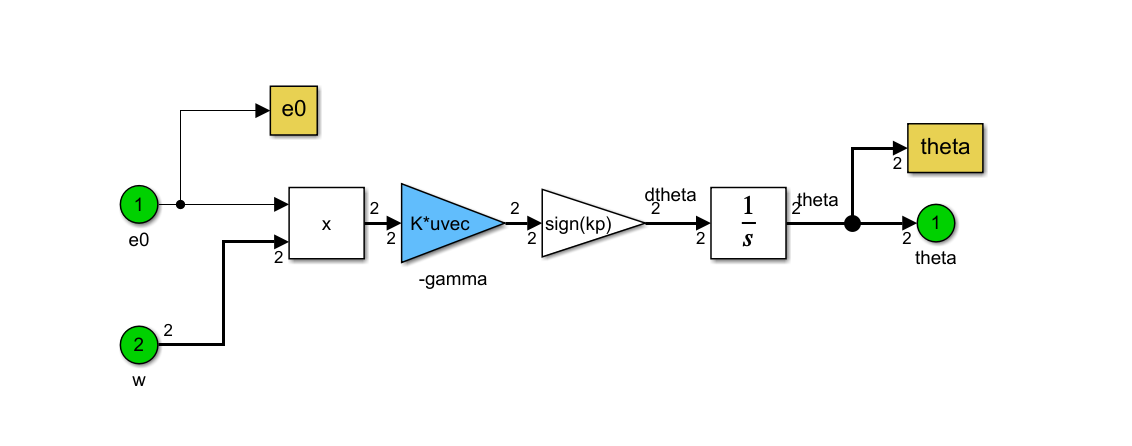
\includegraphics[width=0.6\textwidth]{img/diagrama_adaptacao.png}
  \caption{Malha de adaptação dos parâmetros $\bm{\theta}$.}
  \label{fig:adaptacao}
\end{figure}

Na Figura~\ref{fig:adaptacao}, destacamos a malha de adaptação, responsável por ajustar os parâmetros do controlador $\bm{\theta}$ com base no erro de seguimento. Essa adaptação ocorre conforme uma lei de atualização derivada da função de Lyapunov, garantindo estabilidade do sistema.

\begin{figure}[h!]
  \centering
  \begin{subfigure}[b]{0.32\textwidth}
    \centering
    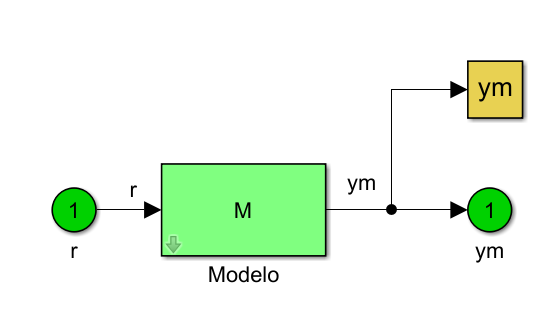
\includegraphics[width=\textwidth]{img/diagrama_modelo.png}
    \caption{Modelo de referência}
    \label{fig:modelo_referencia}
  \end{subfigure}
  \hfill
  \begin{subfigure}[b]{0.32\textwidth}
    \centering
    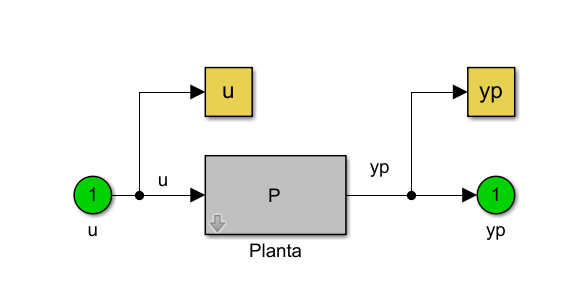
\includegraphics[width=\textwidth]{img/diagrama_planta.png}
    \caption{Planta controlada}
    \label{fig:planta}
  \end{subfigure}
  \hfill
  \begin{subfigure}[b]{0.32\textwidth}
    \centering
    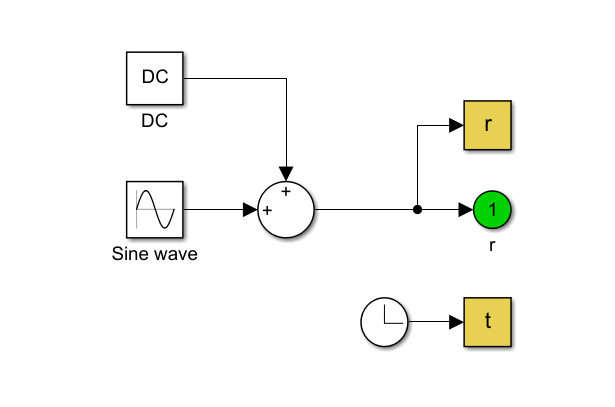
\includegraphics[width=\textwidth]{img/diagrama_referencia.png}
    \caption{Sinal de referência $r(t)$}
    \label{fig:referencia}
  \end{subfigure}
  \caption{Componentes individuais do sistema MRAC.}
  \label{fig:componentes_mrac}
\end{figure}

A Figura~\ref{fig:componentes_mrac} agrupa os blocos fundamentais do sistema MRAC. À esquerda, o modelo de referência define a dinâmica desejada para o sistema. Ao centro, está a planta controlada, que deve seguir essa referência. À direita, o sinal de referência $r(t)$ atua como entrada comum para ambos os blocos, sendo a base para comparação entre o comportamento ideal e o real.

\section{Resultados das simulações}

Cada subseção a seguir apresenta a configuração do experimento, espaço reservado para os dados obtidos em cada simulação e comentários sobre o desempenho do MRAC Direto.

%---------------------------------------------------------------------
\subsection{Simulação \#1}
\paragraph{Configuração do experimento:}
\begin{itemize}
\item \textbf{Planta:} $P(s) = \dfrac{k_p}{s - a_p} = \dfrac{1}{s - 2}$
\item \textbf{Modelo de referência:} $M(s) = \dfrac{k_m}{s + a_m} = \dfrac{1}{s + 1}$
\item \textbf{Condições iniciais:} $y_p(0)=0$, $y_m(0)=0$
\item \textbf{Sinal de referência:} DC = 1 (constante), $A_s=0$, $\omega_s=5$,rad/s
\item \textbf{Ganho de matching ótimo:} $\theta^* = \bigl[-(a_p + a_m)/k_p;;k_m/k_p\bigr] = [-3;,1]$
\item \textbf{Ganho de adaptação:} $\Gamma_1 = 2I_{2\times2}$, $\Gamma_2 = 100 I_{2\times2}$
\item \textbf{Condição inicial do parâmetro:} $\theta(0) = [0;,0]$
\end{itemize}

\paragraph{Resultados da simulação:}
% (incluir gráficos de $y_p$, $y_m$, parâmetros, erro, etc.)
\vspace{2em}

\paragraph{Comentários:}
% - Ajuste inicial do erro de rastreamento; \newline
% - Convergência dos parâmetros para valores próximos a $\theta^*$; \newline
% - Comportamento em regime permanente.

%---------------------------------------------------------------------
\subsection{Simulação \#2}
\paragraph{Configuração do experimento:}
\begin{itemize}
\item \textbf{Planta:} $P(s) = \dfrac{1}{s - 2}$
\item \textbf{Modelo de referência:} $M(s) = \dfrac{1}{s + 1}$
\item \textbf{Condições iniciais:} $y_p(0)=0$, $y_m(0)=0$
\item \textbf{Sinal de referência:} DC = 2 (constante), $A_s=1$, $\omega_s=5$,rad/s
\item \textbf{Ganho de matching ótimo:} $\theta^* = [-3;,1]$
\item \textbf{Ganho de adaptação:} $\Gamma_1 = 2I_{2\times2}$, $\Gamma_2 = 100 I_{2\times2}$
\item \textbf{Condição inicial do parâmetro:} $\theta(0) = [0;,0]$
\end{itemize}

\paragraph{Resultados da simulação:}
% (incluir gráficos de resposta ao degrau + senoide)
\vspace{2em}

\paragraph{Comentários:}
% - Influência da componente senoide no rastreamento; \newline
% - Oscilações residuais em regime permanente.

%---------------------------------------------------------------------
\subsection{Simulação \#3}
\paragraph{Configuração do experimento:}
\begin{itemize}
\item \textbf{Planta:} $P(s) = \dfrac{1}{s - 2}$
\item \textbf{Modelo de referência:} $M(s) = \dfrac{1}{s + 1}$
\item \textbf{Condições iniciais:} $y_p(0)=3$, $y_m(0)=0$
\item \textbf{Sinal de referência:} DC = 1 (constante), $A_s=0$, $\omega_s=5$,rad/s
\item \textbf{Ganho de matching ótimo:} $\theta^* = [-3;,1]$
\item \textbf{Ganho de adaptação:} $\Gamma_1 = 2I_{2\times2}$, $\Gamma_2 = 100 I_{2\times2}$
\item \textbf{Condição inicial do parâmetro:} $\theta(0) = [0;,0]$
\end{itemize}

\paragraph{Resultados da simulação:}
% (incluir levantamento inicial da planta e convergência)
\vspace{2em}

\paragraph{Comentários:}
% - Efeito do deslocamento inicial em $y_p$; \newline
% - Ajuste rápido do erro de rastreamento.

%---------------------------------------------------------------------
\subsection{Simulação \#4}
\paragraph{Configuração do experimento:}
\begin{itemize}
\item \textbf{Planta:} $P(s) = \dfrac{1}{s - 2}$
\item \textbf{Modelo de referência:} $M(s) = \dfrac{1}{s + 1}$
\item \textbf{Condições iniciais:} $y_p(0)=3$, $y_m(0)=0$
\item \textbf{Sinal de referência:} DC = 2 (constante), $A_s=1$, $\omega_s=5$,rad/s
\item \textbf{Ganho de matching ótimo:} $\theta^* = [-3;,1]$
\item \textbf{Ganho de adaptação:} $\Gamma_1 = 2I_{2\times2}$, $\Gamma_2 = 100 I_{2\times2}$
\item \textbf{Condição inicial do parâmetro:} $\theta(0) = [0;,0]$
\end{itemize}

\paragraph{Resultados da simulação:}
% (incluir resposta ao degrau + senoide com deslocamento inicial)
\vspace{2em}

\paragraph{Comentários:}
% - Combinação de deslocamento e referência variável; \newline
% - Desempenho comparado à Simulação #2.

%---------------------------------------------------------------------
\subsection{Simulação \#5}
\paragraph{Configuração do experimento:}
\begin{itemize}
\item \textbf{Planta:} $P(s) = \dfrac{1}{s - 2}$
\item \textbf{Modelo de referência:} $M(s) = \dfrac{1}{s + 4}$
\item \textbf{Condições iniciais:} $y_p(0)=0$, $y_m(0)=0$
\item \textbf{Sinal de referência:} DC = 1 (constante), $A_s=0$, $\omega_s=5$,rad/s
\item \textbf{Ganho de matching ótimo:} $\theta^* = [-(2+4)/1;,1/1] = [-6;,1]$
\item \textbf{Ganho de adaptação:} $\Gamma_1 = 2I_{2\times2}$, $\Gamma_2 = 100 I_{2\times2}$
\item \textbf{Condição inicial do parâmetro:} $\theta(0) = [0;,0]$
\end{itemize}

\paragraph{Resultados da simulação:}
% (incluir análise de modelo de referência mais rápido)
\vspace{2em}

\paragraph{Comentários:}
% - Resposta comparada às simulações anteriores; \newline
% - Impacto do pólo do modelo de referência em $a_m=4$.

\subsection{Simulação \#6}
\paragraph{Configuração do experimento:}
\begin{itemize}
\item \textbf{Planta:} $P(s) = \dfrac{1}{s - 2}$
\item \textbf{Modelo de referência:} $M(s) = \dfrac{1}{s + 4}$
\item \textbf{Condições iniciais:} $y_p(0)=0$, $y_m(0)=0$
\item \textbf{Sinal de referência:} DC = 2, $A_s=1$, $\omega_s=5$ rad/s
\item \textbf{Ganho de matching ótimo:} $\theta^* = [-(2+4)/1;;2/1] = [-6;;2]$
\item \textbf{Ganho de adaptação:} $\Gamma_1 = 2I_{2\times2}$, $\Gamma_2 = 100I_{2\times2}$
\item \textbf{Condição inicial do parâmetro:} $\theta(0) = [0;;0]$
\end{itemize}

\paragraph{Resultados da simulação:}
\vspace{2em}

\paragraph{Comentários:}
% - Sinal de referência composto por componente constante e senoidal
% - Modelo de referência mais rápido ($a_m = 4$)

\subsection{Simulação \#7}
\paragraph{Configuração do experimento:}
\begin{itemize}
\item \textbf{Planta:} $P(s) = \dfrac{1}{s - 2}$
\item \textbf{Modelo de referência:} $M(s) = \dfrac{2}{s + 1}$
\item \textbf{Condições iniciais:} $y_p(0)=0$, $y_m(0)=0$
\item \textbf{Sinal de referência:} DC = 1, $A_s=0$, $\omega_s=5$ rad/s
\item \textbf{Ganho de matching ótimo:} $\theta^* = [-(2+1)/1;;2/1] = [-3;;2]$
\item \textbf{Ganho de adaptação:} $\Gamma_1 = 2I_{2\times2}$, $\Gamma_2 = 100I_{2\times2}$
\item \textbf{Condição inicial do parâmetro:} $\theta(0) = [0;;0]$
\end{itemize}

\paragraph{Resultados da simulação:}
\vspace{2em}

\paragraph{Comentários:}
% - Modelo de referência mais lento do que em simulações anteriores
% - Sinal de referência puramente constante

\subsection{Simulação \#8}
\paragraph{Configuração do experimento:}
\begin{itemize}
\item \textbf{Planta:} $P(s) = \dfrac{1}{s - 2}$
\item \textbf{Modelo de referência:} $M(s) = \dfrac{2}{s + 1}$
\item \textbf{Condições iniciais:} $y_p(0)=0$, $y_m(0)=0$
\item \textbf{Sinal de referência:} DC = 2, $A_s=1$, $\omega_s=5$ rad/s
\item \textbf{Ganho de matching ótimo:} $\theta^* = [-(2+1)/1;;2/1] = [-3;;2]$
\item \textbf{Ganho de adaptação:} $\Gamma_1 = 2I_{2\times2}$, $\Gamma_2 = 100I_{2\times2}$
\item \textbf{Condição inicial do parâmetro:} $\theta(0) = [0;;0]$
\end{itemize}

\paragraph{Resultados da simulação:}
\vspace{2em}

\paragraph{Comentários:}
% - Sinal de referência misto (DC + senoide)
% - Mesmo modelo de referência da simulação anterior

\subsection{Simulação \#9}
\paragraph{Configuração do experimento:}
\begin{itemize}
\item \textbf{Planta:} $P(s) = \dfrac{1}{s - 2}$
\item \textbf{Modelo de referência:} $M(s) = \dfrac{1}{s + 1}$
\item \textbf{Condições iniciais:} $y_p(0)=0$, $y_m(0)=0$
\item \textbf{Sinal de referência:} DC = 1, $A_s=0$, $\omega_s=5$ rad/s
\item \textbf{Ganho de matching ótimo:} $\theta^* = [-(2+1)/1;;1/1] = [-3;;1]$
\item \textbf{Ganho de adaptação:} 
\[
\Gamma_1 = 2 \begin{bmatrix} 1 & 0.35 \\ 0.35 & 1 \end{bmatrix}, \quad
\Gamma_2 = 100 \begin{bmatrix} 1 & 0.35 \\ 0.35 & 1 \end{bmatrix}
\]
\item \textbf{Condição inicial do parâmetro:} $\theta(0) = [0;;0]$
\end{itemize}

\paragraph{Resultados da simulação:}
\vspace{2em}

\paragraph{Comentários:}
% - Mudança na matriz de ganho de adaptação (matriz não-diagonal)
% - Sinal de referência puramente constante

\subsection{Simulação \#10}
\paragraph{Configuração do experimento:}
\begin{itemize}
\item \textbf{Planta:} $P(s) = \dfrac{1}{s - 2}$
\item \textbf{Modelo de referência:} $M(s) = \dfrac{1}{s + 1}$
\item \textbf{Condições iniciais:} $y_p(0)=0$, $y_m(0)=0$
\item \textbf{Sinal de referência:} DC = 2, $A_s=1$, $\omega_s=5$ rad/s
\item \textbf{Ganho de matching ótimo:} $\theta^* = [-(2+1)/1;;1/1] = [-3;;1]$
\item \textbf{Ganho de adaptação:} 
\[
\Gamma_1 = 2 \begin{bmatrix} 1 & 0.35 \\ 0.35 & 1 \end{bmatrix}, \quad
\Gamma_2 = 100 \begin{bmatrix} 1 & 0.35 \\ 0.35 & 1 \end{bmatrix}
\]
\item \textbf{Condição inicial do parâmetro:} $\theta(0) = [0;;0]$
\end{itemize}

\paragraph{Resultados da simulação:}
\vspace{2em}

\paragraph{Comentários:}
% - Mesma estrutura de adaptação da simulação anterior
% - Presença de componente oscilatória no sinal de referência

\end{document}
